\documentclass[12pt,notitlepage]{article}

% for margins
\usepackage[a4paper,left=3cm,right=2cm,top=2.5cm,bottom=2.5cm]{geometry}
% for citations
\usepackage{apacite}
% for hyperlinks
\usepackage{hyperref}
% for maths symbols like the real numbers
\usepackage{amssymb}
\usepackage{graphicx}

\begin{document}



\begin{document}
\bibliographystyle{apacite}

\title{\Large{\textbf{Assignment 7}}}
\date{Novemeber 1, 2020}
\author{Simon Ward-Jones\\simonwardjones16@gmail.com}

\section{Summary}
\begin{itemize}
   \item I decided to explore the cats-dogs-pandas data set: \\https://www.kaggle.com/ashishsaxena2209/animal-image-datasetdog-cat-and-panda
   \item The full notebook where I loaded the data, built an alexnet model and predicted a sample can be explored here: \\ https://colab.research.google.com/github/simonwardjones/d2l-study-group/blob/master/exercises/assignment-7-sw-j.ipynb
\end{itemize}

\section{Steps in notebook}
\begin{enumerate}
  \item[1] Connect to kaggle api and download data
  \begin{enumerate}
    \item Mount Google drive
    \item Install kaggle cli then download and unzip data
  \end{enumerate}
  \item[2] Explore the data and prepare dataset/dataloader
  \begin{enumerate}
    \item Use the torchvision datasets.ImageFolder helper to define dataset
    \item Use torchvision Resize transformer and visually inspect a few samples
  \end{enumerate}
  \item[3] Train test split data
  \begin{enumerate}
    \item Use sklearn train\_test\_split to stratify (same proportion of animals in train and test)
    \item Define batch\_size, learning rate and num epochs
    \item Create data loaders for train/test using SubsetRandomSampler
    \item use Resize and ToTensor transforms
    \item Note a batch has size [64, 3, 224, 224] 64 samples, 3 input channels, height and width 224
  \end{enumerate}
  \item[4] Define AlexNet structure
  \begin{enumerate}
    \item I used the same architecture as alex net 
    \begin{figure}
      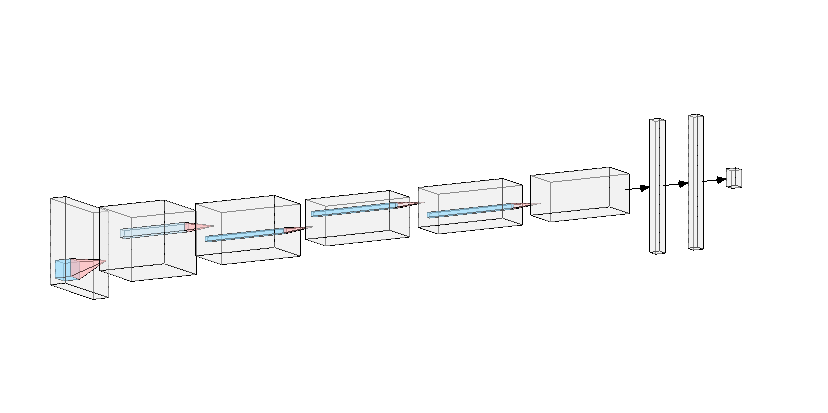
\includegraphics[width=\linewidth]{alexnet.png}
      \caption{AlexNet architecture}
      \label{fig:AlexNet architecture}
    \end{figure} 
    \item Throughout the net channels increase as height and width decrease using sequential convolutions (of decreasing kernel sizes) and max pooling (after 1st, 2nd and 5th convolutions). 
    \item The Relu activation is used throughout after each convolution and before maxpooling 
    \item The final three layers are fully connected
  \end{enumerate}
  \item[4] Train model
  \begin{enumerate}
    \item Train model using animator to visulalise loss and test accuracy
    \item If already trained load from gdrive
    \item Save the model using torch. Save and cp to drive 
  \end{enumerate}
  \item[4] Predict examples
  \begin{enumerate}
    \item Predict examples and show images
  \end{enumerate}
\end{enumerate}



\vfill
\bibliography{../References}
\nocite{zhang2020dive}
\end{document}

